\documentclass[10pt, a4paper]{article}
\usepackage{geometry}
\geometry{a4paper,total={6in, 8in}, margin=0.25in}
\usepackage{booktabs}
\usepackage{courier}
\usepackage{amssymb}
\usepackage{fourier}
\usepackage{color}
\usepackage{graphicx}
\DeclareGraphicsExtensions{.png}
\usepackage{tikz-timing}
\usepackage{scalerel}
\usepackage{stackengine}

\newcommand\showdiv[1]{\overline{\smash{\hstretch{.5}{)}\mkern-3.2mu\hstretch{.5}{)}}#1}}
\newcommand\ph[1]{\textcolor{white}{#1}}

\begin{document}

\begin{enumerate}
\item\mbox{}
    \begin{enumerate}
    \item\mbox{}\\
        Achieve at 4800 baud means 4800 symbols per second.\\
        Each symbol contains $\log_2 4 = 2$ bits\\
        Data rate $= 2 \times 4800 = 9600 (bps)$
    \item\mbox{}\\
        $\because \left(2, 3\right) \times 3 = \left(6, 9\right)$\\
        $\Rightarrow \left(2, 3\right) \parallelslant \left(6, 9\right)$\\
        $\Rightarrow$ There is only amplitude difference but phase difference between $\left(2, 3\right)$ and $\left(6, 9\right)$\\
        $\therefore$ The modem uses amplitude modulation
    \end{enumerate}

\item\mbox{}
    \begin{enumerate}
    \item\mbox{}\\
        Translate the data bit sequence into decimal sequence:
        %$$0000\ 1100\ 1111\ 1111\ 0101\ 0000$$
        %$$0110\ 0000\ 1111\ 1111\ 0000\ 1100$$
        %$$\Downarrow$$
        $$12\qquad 255\qquad 80$$
        $$96\qquad 255\qquad 12$$
        Replace 12 with DLE, 2 with STX, and ETX with 1:
        $$DLE\qquad 255\qquad 80\qquad 96\qquad 255\qquad DLE$$
        Prefix ETX/DLE with DLE:\@
        $$\textcolor{red}{DLE}\qquad DLE\qquad 255\qquad 80\qquad 96\qquad 255\qquad \textcolor{red}{DLE}\qquad DLE$$
        Add STX at the front and ETX at the end:
        $$\textcolor{blue}{STX}\qquad \textcolor{red}{DLE}\qquad DLE\qquad 255\qquad 80\qquad 96\qquad 255\qquad \textcolor{red}{DLE}\qquad DLE\qquad \textcolor{blue}{ETX}$$
        Translate decimal sequence back to bit sequence:
        $$\textcolor{blue}{0000\ 0010}\ \textcolor{red}{0000\ 1100}\ 0000\ 1100\ 1111\ 1111\ 0101\ 0000$$
        $$0110\ 0000\ 1111\ 1111\ \textcolor{red}{0000\ 1100}\ 0000\ 1100\ \textcolor{blue}{0000\ 0001}$$
    \item\mbox{}\\
        Insert 0 after pattern 011111:
        %$$0000\ 1100\ 1111\ 1111\ 0101\ 0000$$
        %$$0110\ 0000\ 1111\ 1111\ 0000\ 1100$$
        %$$\Downarrow$$
        $$0000\ 1100\ 1111\ 1\textcolor{red}{0}111\ 0101\ 0000$$
        $$0110\ 0000\ 1111\ 1\textcolor{red}{0}111\ 0000\ 1100$$
        Add frame marker 01111110 at both front and end:
        $$\textcolor{blue}{0111\ 1110}\ 0000\ 1100\ 1111\ 1\textcolor{red}{0}111\ 0101\ 0000$$
        $$0110\ 0000\ 1111\ 1\textcolor{red}{0}111\ 0000\ 1100\ \textcolor{blue}{0111\ 1110}$$
    \item\mbox{}\\
        Add a start bit ``1'' and an end bit ``0'' for every 8-bit characters:
        $$\textcolor{blue}{1}0000\ 1100\textcolor{blue}{0}\ \textcolor{blue}{1}1111\ 1111\textcolor{blue}{0}\ \textcolor{blue}{1}0101\ 0000\textcolor{blue}{0}$$
        $$\textcolor{blue}{1}0110\ 0000\textcolor{blue}{0}\ \textcolor{blue}{1}1111\ 1111\textcolor{blue}{0}\ \textcolor{blue}{1}0000\ 1100\textcolor{blue}{0}$$
    \item\mbox{}\\
        Efficiency of BISYNC protocol $= \frac{48}{48 + 32} = 0.6 = 60 \%$\\
        Efficiency of HDLC protocol $= \frac{48}{48 + 18} \simeq 0.727 = 72.7 \%$\\
        Efficiency of 8-bit RS-232 $= \frac{48}{48 + 12} = 0.8 = 80 \%$
    \end{enumerate}

\item\mbox{}
    \begin{enumerate}
    \item\mbox{}\\
    \begin{tikztimingtable}[timing/slope=0,xscale=1.4,yscale=1.5]
        Bits & 2D{0}2D{1}2D{0}2D{1}2D{1}2D{1}2D{1}2D{1}2D{0}2D{0}2D{0}2D{1}2D{1}2D{0}2D{1}2D{1}\\
        NRZ & LLHHLLHHHHHHHHHHLLLLLLHHHHLLHHHH\\
        Clock & 32{C}\\
        Manchester & LHHLLHHLHLHLHLHLLHLHLHHLHLLHHLHL\\
        NRZI & LLLHHHHLLHHLLHHLLLLLLLLHHLLLLHHL\\
    \extracode
        \begin{pgfonlayer}{background}
            \begin{scope}[gray,semitransparent]
                \horlines{2,3,4,5}
                \vertlines[dashed]{0,2,...,32}
            \end{scope}
        \end{pgfonlayer}
    \end{tikztimingtable}\\

    \begin{tikztimingtable}[timing/slope=0,xscale=1.4,yscale=1.5]
        Bits & 2D{0}2D{1}2D{0}2D{1}2D{1}2D{1}2D{1}2D{1}2D{0}2D{1}2D{0}2D{1}2D{0}2D{0}2D{1}2D{1}2D{0}2D{1}2D{1}2D{1}\\
        %Clock & 40{C}\\
        4B/5B & LLLHHHHLLHHLLHHLLLLHHHHLLLLLLHHLLLLHHLLH\\
    \extracode
        \begin{pgfonlayer}{background}
            \begin{scope}[gray,semitransparent]
                \horlines{2}
                \vertlines[dashed]{0,2,...,40}
            \end{scope}
        \end{pgfonlayer}
    \end{tikztimingtable}
    \item\mbox{}\\
        $\mbox{channel capacity}\ C = B \log_2\left(1 + SNR\right)$\\
        $44.736 \times 10^6 \leq \mbox{channel capacity}\ C = 25 \times 10^6 \times \log_2\left(1 + SNR\right)$\\
        $\Rightarrow \log_2\left(1 + SNR\right) \geq \frac{44.736}{25}$\\
        $\Rightarrow SNR \geq 2^{\frac{44.736}{25}} - 1 \simeq 2.46$\\
        $= 10 \times \log\left(2.46\right) \mbox{(dB)} \simeq 3.91 \mbox{(dB)}$
    \end{enumerate}

\item\mbox{}
    \begin{enumerate}
    \item\mbox{}\\
        \textcolor{red}{Case 1}, bit 7 error occurs during the transmission:\\
        $\left\{
            \begin{array}{ll}
                C\left(x\right) & = 11011\\
                M\left(x\right) & = 10110110100\\
                k & = 4
            \end{array}
        \right.$\\
        $\Rightarrow T\left(x\right) = M\left(x\right) \times x^k = 101101101000000$\\

        \stackMath\def\stackalignment{r}
        \stackunder{11011 \stackon[1pt]{\showdiv{101101101000000}}{}}{
            \Shortstack[l]{
                {\underline{11011}}
                \ph{1}11011
                {\ph{1}\underline{11011}}
                \ph{123456}10100
                {\ph{123456}\underline{11011}}
                \ph{1234567}11110
                {\ph{1234567}\underline{11011}}
                \ph{123456789}10100
                {\ph{123456789}\underline{11011}}
                \ph{1234567890}11110
                {\ph{1234567890}\underline{11011}}
                \ph{123456789012}101
            }
        }\\
        $R\left(x\right)$ is the remainder from $T\left(x\right) / C\left(x\right)$\\
        $\Rightarrow R\left(x\right) = 101$\\
        The code word $P\left(x\right) = T\left(x\right) - R\left(x\right) = 101101101000101$\\
        Bit 7 error (counting from the least significant bit):
        $$10110110\textcolor{blue}{1}000101 \Rightarrow 10110110\textcolor{red}{0}000101$$
        The error is detected by dividing the received polynomial $\left(P\left(x\right) + E\left(x\right)\right)$ with $C\left(x\right)$\\
        If there is no error, then the remainder must be 0\\

        \stackMath\def\stackalignment{r}
        \stackunder{11011 \stackon[1pt]{\showdiv{101101100000101}}{}}{
            \Shortstack[l]{
                {\underline{11011}}
                \ph{1}11011
                {\ph{1}\underline{11011}}
                \ph{123456}10000
                {\ph{123456}\underline{11011}}
                \ph{1234567}10110
                {\ph{1234567}\underline{11011}}
                \ph{12345678}11011
                {\ph{12345678}\underline{11011}}
                \ph{12345678901234}1
            }
        }\\
        In this case,\\
        $\because \mbox{The remainder of} \left(P\left(x\right) + E\left(x\right)\right) / C\left(x\right) = 1 \neq 0$\\
        $\therefore E\left(x\right) \neq 0 \Rightarrow$ Error generated during transmission\\
        $\Rightarrow$ Detect the error occurs during the transmission\\

        \textcolor{red}{Case 2}, bit 7 error occurs before the transmission:\\
        $\left\{
            \begin{array}{ll}
                C\left(x\right) & = 11011\\
                M\left(x\right) & = 1011\textcolor{blue}{0}110100 \Rightarrow 1011\textcolor{red}{1}110100\\
                k & = 4
            \end{array}
        \right.$\\
        $\Rightarrow T\left(x\right) = M\left(x\right) \times x^k = 101111101000000$\\

        \stackMath\def\stackalignment{r}
        \stackunder{11011 \stackon[1pt]{\showdiv{101111101000000}}{}}{
            \Shortstack[l]{
                {\underline{11011}}
                \ph{1}11001
                {\ph{1}\underline{11011}}
                \ph{1234}10101
                {\ph{1234}\underline{11011}}
                \ph{12345}11100
                {\ph{12345}\underline{11011}}
                \ph{1234567}11100
                {\ph{1234567}\underline{11011}}
                \ph{123456789}11100
                {\ph{123456789}\underline{11011}}
                \ph{12345678901}1110
            }
        }\\
        $R\left(x\right)$ is the remainder from $T\left(x\right) / C\left(x\right)$\\
        $\Rightarrow R\left(x\right) = 1110$\\
        The code word $P\left(x\right) = T\left(x\right) - R\left(x\right) = 101111101001110$\\

        \stackMath\def\stackalignment{r}
        \stackunder{11011 \stackon[1pt]{\showdiv{101111101001110}}{}}{
            \Shortstack[l]{
                {\underline{11011}}
                \ph{1}11001
                {\ph{1}\underline{11011}}
                \ph{1234}10101
                {\ph{1234}\underline{11011}}
                \ph{12345}11100
                {\ph{12345}\underline{11011}}
                \ph{1234567}11101
                {\ph{1234567}\underline{11011}}
                \ph{123456789}11011
                {\ph{123456789}\underline{11011}}
                \ph{12345678901234}0
            }
        }\\
        In this case,\\
        The error cannot be detected by dividing the received polynomial $\left(P\left(x\right) + E\left(x\right)\right)$ with $C\left(x\right)$\\
    $\because \mbox{The remainder of} \left(P\left(x\right) + E\left(x\right)\right) / C\left(x\right) = 0$\\
        $\therefore E\left(x\right) = 0 \Rightarrow$ No error generated during transmission\\
        $\Rightarrow$ Cannot detect the error occurs before the transmission
    \item\mbox{}\\
        $\left\{
            \begin{array}{ll}
                C\left(x\right) & = 11011\\
                P\left(x\right) + E\left(x\right) & = 10010110011\\
                k & = 4
            \end{array}
        \right.$\\

        \stackMath\def\stackalignment{r}
        \stackunder{11011 \stackon[1pt]{\showdiv{10010110011}}{}}{
            \Shortstack[l]{
                {\underline{11011}}
                \ph{1}10011
                {\ph{1}\underline{11011}}
                \ph{12}10001
                {\ph{12}\underline{11011}}
                \ph{123}10100
                {\ph{123}\underline{11011}}
                \ph{1234}11110
                {\ph{1234}\underline{11011}}
                \ph{123456}10111
                {\ph{123456}\underline{11011}}
                \ph{1234567}1100
            }
        }\\
        $\because \mbox{The remainder of} \left(P\left(x\right) + E\left(x\right)\right) / C\left(x\right) = 1100 \neq 0$\\
        $\therefore E\left(x\right) \neq 0 \Rightarrow$ Error generated during transmission
    \end{enumerate}

\item\mbox{}
    \begin{enumerate}
    \item\mbox{}\\
        \colorbox{black}{\textcolor{white}{\$ \texttt{ss -or `sport = :ssh or dport = :ssh' | less}}}\\
        First 3 lines of output:\\
        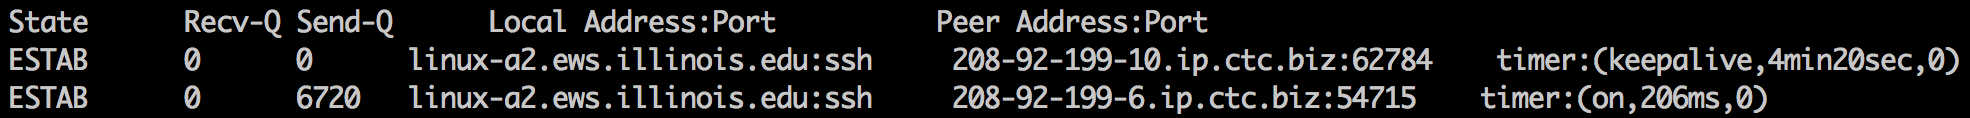
\includegraphics[width=6.5in]{images/ss_output}\\

        \colorbox{black}{\textcolor{white}{\$ \texttt{ss -o `sport = :ssh or dport = :ssh' | less}}}\\
        First 3 lines of output:\\
        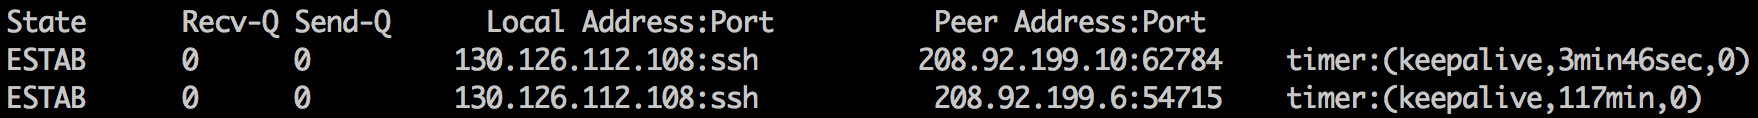
\includegraphics[width=6.5in]{images/ss_output_ip}
    \item\mbox{}\\
        All linux5, linux6, and linux7 redirect to the same machine, so they have the same Ethernet Address and the same IP Address.\\

        linux5:\\
        \colorbox{black}{\textcolor{white}{\$ \texttt{ping -c 1 linux5.ews.illinois.edu}}}\\
        \colorbox{black}{\textcolor{white}{\$ \texttt{arp -a linux5.ews.illinois.edu}}}\\
        Output:\\
        \colorbox{black}{\textcolor{white}{\texttt{linux-v1.ews.illinois.edu (130.126.112.107) at 00:50:56:bd:00:9e [ether] on eth0}}}\\

        linux6:\\
        \colorbox{black}{\textcolor{white}{\$ \texttt{ping -c 1 linux6.ews.illinois.edu}}}\\
        \colorbox{black}{\textcolor{white}{\$ \texttt{arp -a linux6.ews.illinois.edu}}}\\
        Output:\\
        \colorbox{black}{\textcolor{white}{\texttt{linux-v1.ews.illinois.edu (130.126.112.107) at 00:50:56:bd:00:9e [ether] on eth0}}}\\

        linux7:\\
        \colorbox{black}{\textcolor{white}{\$ \texttt{ping -c 1 linux7.ews.illinois.edu}}}\\
        \colorbox{black}{\textcolor{white}{\$ \texttt{arp -a linux7.ews.illinois.edu}}}\\
        Output:\\
        \colorbox{black}{\textcolor{white}{\texttt{linux-v1.ews.illinois.edu (130.126.112.107) at 00:50:56:bd:00:9e [ether] on eth0}}}\\

        \begin{tabular}{ll}
        \toprule
        Machine & Ethernet Address\\
        \midrule
        linux5 & \texttt{00:50:56:bd:00:9e}\\
        linux6 & \texttt{00:50:56:bd:00:9e}\\
        linux7 & \texttt{00:50:56:bd:00:9e}\\
        \bottomrule
        \end{tabular}
    \item\mbox{}\\
        Hardware Address: \texttt{D4:AE:52:AA:DB:E6}\\
        Hostname: \texttt{linux-a2.ews.illinois.edu}
    \end{enumerate}
\end{enumerate}

\end{document}
